\documentclass[border=4pt]{standalone}
\usepackage{tikz}
\usetikzlibrary{arrows.meta, positioning, fit, backgrounds, calc}
\usepackage{xcolor}

% Brand colors
\definecolor{garnet}{HTML}{73000A}
\definecolor{atlantic}{HTML}{466A9F}
\definecolor{congaree}{HTML}{1F414D}
\definecolor{black90}{HTML}{363636}
\definecolor{black70}{HTML}{5C5C5C}
\definecolor{black30}{HTML}{C7C7C7}
\definecolor{black10}{HTML}{ECECEC}

\begin{document}
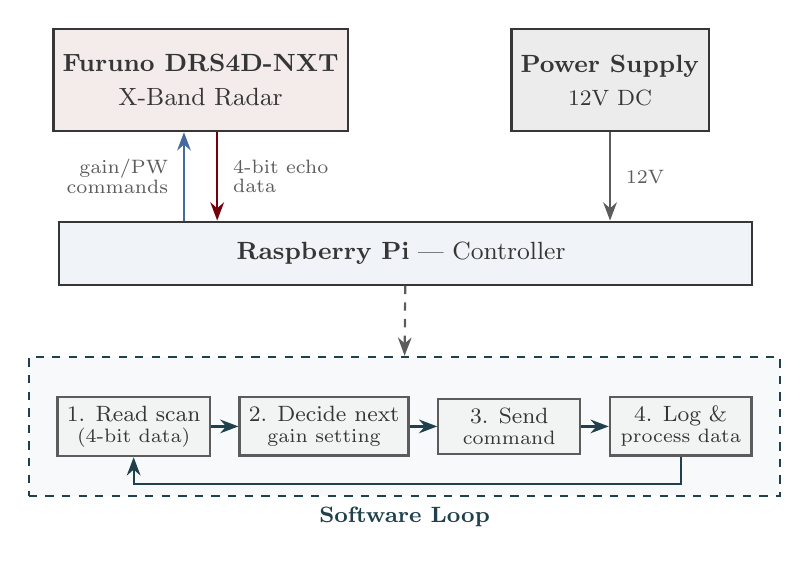
\begin{tikzpicture}[
    >=Stealth,
    box/.style={
        draw=black90,
        thick,
        minimum height=1.3cm,
        align=center,
        font=\small,
        text=black90,
    },
    stepbox/.style={
        draw=black70,
        thick,
        minimum width=1.8cm,
        minimum height=0.6cm,
        align=center,
        font=\footnotesize,
        text=black90,
        fill=congaree!6,
    },
    lbl/.style={
        font=\scriptsize,
        text=black70,
    },
]

% --- Top row: Radar and Power, placed by coordinates ---
\node[box, fill=garnet!8, minimum width=3.2cm] (radar) at (0,0) {
    \textbf{Furuno DRS4D-NXT}\\[1pt]
    X-Band Radar
};

\node[box, fill=black10, minimum width=2.4cm] (power) at (5.2,0) {
    \textbf{Power Supply}\\[1pt]
    {\footnotesize 12V DC}
};

% --- Raspberry Pi below, spanning from radar left edge to power right edge ---
\node[box, fill=atlantic!8,
    minimum width=8.8cm,
    minimum height=0.8cm,
] (rpi) at (2.6,-2.2) {
    \textbf{Raspberry Pi} --- Controller
};

% --- Hardware arrows: all vertical ---
% Commands: Pi -> Radar (left arrow)
\draw[->, thick, atlantic]
    ([xshift=-6pt]radar.south |- rpi.north) --
    node[lbl, left=2pt, align=right] {gain/PW\\[-1pt]commands}
    ([xshift=-6pt]radar.south);

% Echo data: Radar -> Pi (right arrow)
\draw[->, thick, garnet]
    ([xshift=6pt]radar.south) --
    node[lbl, right=2pt, align=left] {4-bit echo\\[-1pt]data}
    ([xshift=6pt]radar.south |- rpi.north);

% Power -> Pi: straight down
\draw[->, thick, black70]
    (power.south) --
    node[lbl, right=2pt] {12V}
    (power.south |- rpi.north);

% --- Software loop: single row centered under Pi ---
\node[stepbox] (read) at (-0.85, -4.4) {
    1. Read scan\\[-2pt]
    {\scriptsize(4-bit data)}
};
\node[stepbox, right=0.35cm of read] (decide) {
    2. Decide next\\[-2pt]
    {\scriptsize gain setting}
};
\node[stepbox, right=0.35cm of decide] (send) {
    3. Send\\[-2pt]
    {\scriptsize command}
};
\node[stepbox, right=0.35cm of send] (log) {
    4. Log \&\\[-2pt]
    {\scriptsize process data}
};

% Forward arrows
\draw[->, thick, congaree] (read.east) -- (decide.west);
\draw[->, thick, congaree] (decide.east) -- (send.west);
\draw[->, thick, congaree] (send.east) -- (log.west);
% Return arrow looping underneath
\draw[->, thick, congaree]
    (log.south) -- ++(0,-0.35) -| (read.south);

% Software loop background
\begin{scope}[on background layer]
\node[
    draw=congaree,
    dashed,
    thick,
    fit=(read)(decide)(send)(log),
    inner xsep=10pt,
    inner ysep=14pt,
    fill=congaree!3,
    label={[lbl, text=congaree, font=\footnotesize\bfseries]below:Software Loop},
] (swloop) {};
\end{scope}

% Dashed connection Pi -> Loop
\draw[->, thick, dashed, black70]
    (rpi.south) -- (swloop.north);

\end{tikzpicture}
\end{document}
